%% GENERATED by board/haipipe-board/cli/build-displays.py from
%%   ../display/QBt3-for-display/float.tex
%% Do not edit this file. Edit the copy under ../display/ and rebuild.
\begin{figure}[t]
  \centering
  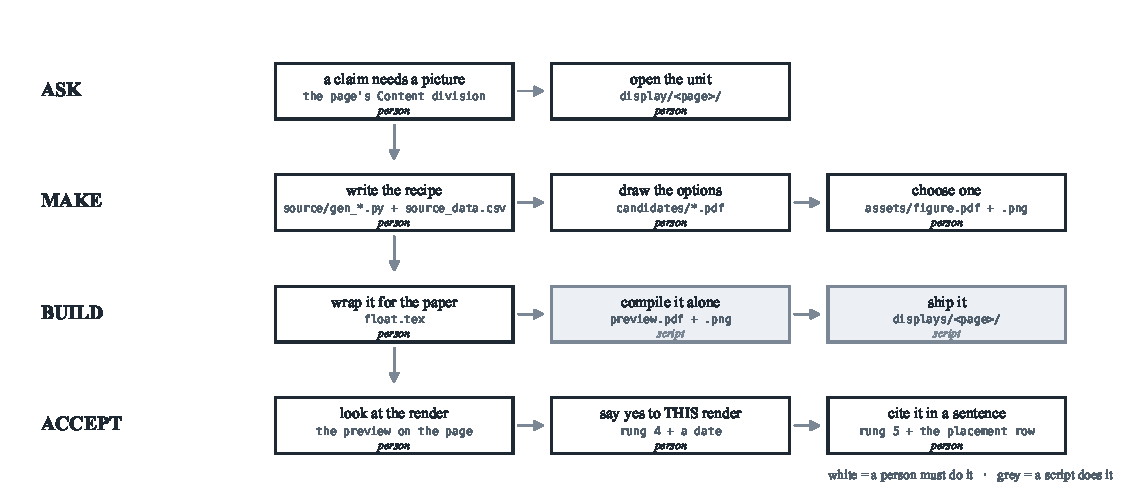
\includegraphics[width=0.95\textwidth]{displays/QBt3-for-display/assets/figure.pdf}
  \caption{How one display unit is produced, and who is allowed to do each step.
  Four lanes, eleven steps, read left to right within a lane and top to bottom
  between them. A white box is a step a person must take; a grey box is a step a
  script takes. Only two of the eleven are grey, and both sit in BUILD: the
  standalone preview compile, and the copy into \texttt{displays/}. Every step in
  ACCEPT is white, which is the rule this figure exists to make visible: a
  machine may render a display and may ship it, and no machine may accept one.
  Drawn from \texttt{source/source\_data.csv} at build time; the lane order is
  the only thing the plotting code hardcodes.}
  \label{fig:display-pipeline}
\end{figure}
